%!TEX root=../main.tex

\section{Introduction} % (fold)
\label{sec:introduction}

We extend our congratulations to \cite{happMultivariateFunctionalPrincipal2018} for their outstanding article. Despite the substantial interest on the topic of dimension reduction in the (multivariate) functional data literature, we concur with the authors that existing methods are often limited to either univariate functional data or multivariate functional data defined on a common one-dimensional domain. However, recent research has shown a growing presence of data defined on different dimensional domains, such as curves and surfaces, observed in diverse fields, including neuroscience, biomechanics, and other domains. In this discussion, we aim to provide commentary on the estimation of the number of principal components utilising the methodology devised by the authors. To achieve this, we conducted an extensive simulation study and subsequently propose practical guidelines for practitioners to adeptly chose the appropriate number of components for multivariate functional datasets. For ease of presentation, we use the same notation as theirs. Code to reproduce the simulation study in this discussion is available at \url{https://github.com/FAST-ULxNUIG/variance_mfpca}.

% section introduction (end)

\section{Model} % (fold)
\label{sec:model}

\cite{happMultivariateFunctionalPrincipal2018} proposed an extension of functional principal components analysis (FPCA, \cite{ramsayFunctionalDataAnalysis2005}) to multivariate functional data defined on different dimensional domains, named multivariate functional principal components analysis (MFPCA). We briefly present the estimation procedure of the principal components given a sample $x_1, \dots, x_N$ of multivariate functional data. The detailed estimation procedure is given in \cite[Section 3]{happMultivariateFunctionalPrincipal2018} For all $n = 1, \dots, N$, the observation $x_n$ is a vector of $p$ functions. The first step is to perform a univariate FPCA for each individual feature $j$ using $x_1^{(j)}, \dots, x_N^{(j)}$. We estimate $M_j$ components for each feature $j$. The total number of components that have been estimated is thus $M_+ = \sum_{j = 1}^p M_j$. We also define $M_{-} = \min_{j = 1, \dots, p} M_j$, being the minimum number of univariate components estimated across univariate feature $j$. Using the univariate eigenfunctions, an estimation of the univariate scores is performed, defined as the projection of the curves onto the eigenfunctions. The univariate scores are then concatenated in a matrix of size $N \times M_+$. An eigenanalysis of this matrix is performed resulting in eigenvalues $\nu_m$ and eigenvectors $\mathbf{c}_m$. Finally, the multivariate eigenfunctions and scores are estimated as a linear combination of the univariate eigenfunctions and scores weighted by the eigenvectors $\mathbf{c}_m$. The multivariate eigenvalues are the same as the matrix of the concatenated scores $\nu_m$. In this context, our focus lies in investigating how the selection of the parameter $M_j$ impacts the estimation of the eigenvalues $\nu_m$.

Using this methodology, the number of multivariate eigenvalues that can be estimated is $M_+$. Let $\{\nu_m\}_{1 \leq m \leq M_+}$ be the set of true eigenvalues and $\{\widehat{\nu}_m\}_{1 \leq m \leq M_+}$ be the set of estimated eigenvalues. We use the relative errors $\text{Err}(\widehat{\nu}_m)  = (\nu_m - \widehat{\nu}_m)^2 / \nu^2_m$ to assess the accuracy of the estimates. The authors also claim that the percentage of variance explained is suitable to find appropriate $M_j$ \cite[Chapter 8.2]{ramsayFunctionalDataAnalysis2005}. The percentage of variance explained by the $m$th component and the cumulative percentage of variance explained by the first $m$ components are defined as
\begin{equation}\label{eq:pve}
     \text{PVE}_m = \nu_m \times \left(\sum_{l = 1}^{M_+} \nu_l\right)^{-1}, \quad\text{and}\quad \text{PVE}_{1:m} = \sum_{l = 1}^m \text{PVE}_l, \quad m = 1, \dots, M_+.
\end{equation}
If we fix the percentage of variance explained to be $\alpha\%$, the number of components needed to explain $\alpha\%$ of the variance is given by
\begin{equation}\label{eq:npc}
     \text{NPC}_{\alpha} = \sum_{m = 1}^{M_{+}} \mathbf{1}\left\{\text{PVE}_{1:m} < \alpha\right\} + 1 = \min_{m = 1, \dots, M_+} \text{PVE}_{1:m} > \alpha.
\end{equation}


% section model (end)

\section{Simulation} % (fold)
\label{sec:simulation}

We perform a simulation study based on the first setting in the simulation in \cite{happMultivariateFunctionalPrincipal2018}. The data-generating process is based on a truncated version of the Karhunen-Loève decomposition. First, we generate a large orthonormal basis $\{\psi_m\}_{1 \leq k \leq M}$ of $\sLp{\TT{}}$ on an interval $\TT{} = [0, T] \subset \RR$. We fix $T_1 = 0$ and $T_{p + 1} = T$ and we generate $p - 1$ cutting points $T_2, \dots, T_p$ uniformly in $\TT{}$ such that $0 = T_1 < \cdots < T_p < T_{p+1} = T$. Let $s_1, \dots, s_p \in \{-1, 1\}$ be coefficients that randomly flip the eigenfunctions with probability $0.5$. The univariate components of the eigenfunctions are then defined as
\begin{equation}\label{eq:simulation_uni_component}
    \psi_m^{(j)}(t_j) = s_j \restr{\psi_m}{[T_j, T_{j + 1}]}\left(\frac{t_j - T_j}{T_{j + 1} - T_j}\right), \quad m = 1, \dots, M, \quad j = 1, \dots, p.
\end{equation}
The notation $\restr{\psi_m}{[T_j, T_{j + 1}]}$ is the restriction of the function $\psi_m$ to the set $[T_j, T_{j + 1}]$. The set of multivariate functions $\{\psi_m\}_{1 \leq m \leq M}$ is an orthonormal system in $\HH \coloneqq \sLp{\TT{1}} \times \dots \times \sLp{\TT{p}}$ with $\TT{j} = [0, 1]$. Each curve is then simulated using the truncated multivariate Karhunen-Loève expansion:
\begin{equation}
    x_i(\pointt) = \sum_{m = 1}^M \rho_{i, m} \psi_m(\pointt), \quad \pointt \in \TT{},\quad i = 1, \dots, N,
\end{equation}
where the scores $\rho_{i, m}$ are sampled as random normal variables with mean $0$ and variance $\nu_m$. The eigenvalues $\nu_m$ are defined with an exponential decrease, $\nu_m = \exp(-(m + 1)/2)$. We simulate $N = 25, 50$ and $100$ observations for each replication of the simulation. Similarly, each component is sampled on a regular grid of $S = 25, 50$ and $100$ sampling points. We use $p = 5$ features and we set $M = 50$. The estimation is done using the \textsf{R} package \texttt{MFPCA} (\cite{happ-kurzObjectOrientedSoftwareFunctional2020}). For each univariate feature $j$, we estimate $M_j = 5$ principal components. Then, following the multivariate components estimation procedure, we can estimate $M_+ = 25$ multivariate components. The simulations are replicated $500$ times.

Figure \ref{fig:ncomp} illustrates the obtained results regarding the errors in estimating the eigenvalues. Remarkably, the accuracy of the estimation declines with an increasing number of components in all scenarios. In particular, there is a notable jump in accuracy observed for the last five estimated eigenvalues. Nonetheless, establishing a general rule based on these observations is challenging. We recommend to estimate at most $M_{-}$ multivariate components; otherwise, the univariate components may not contain enough information to effectively recover their corresponding multivariate counterparts.
\begin{figure}
     \centering
    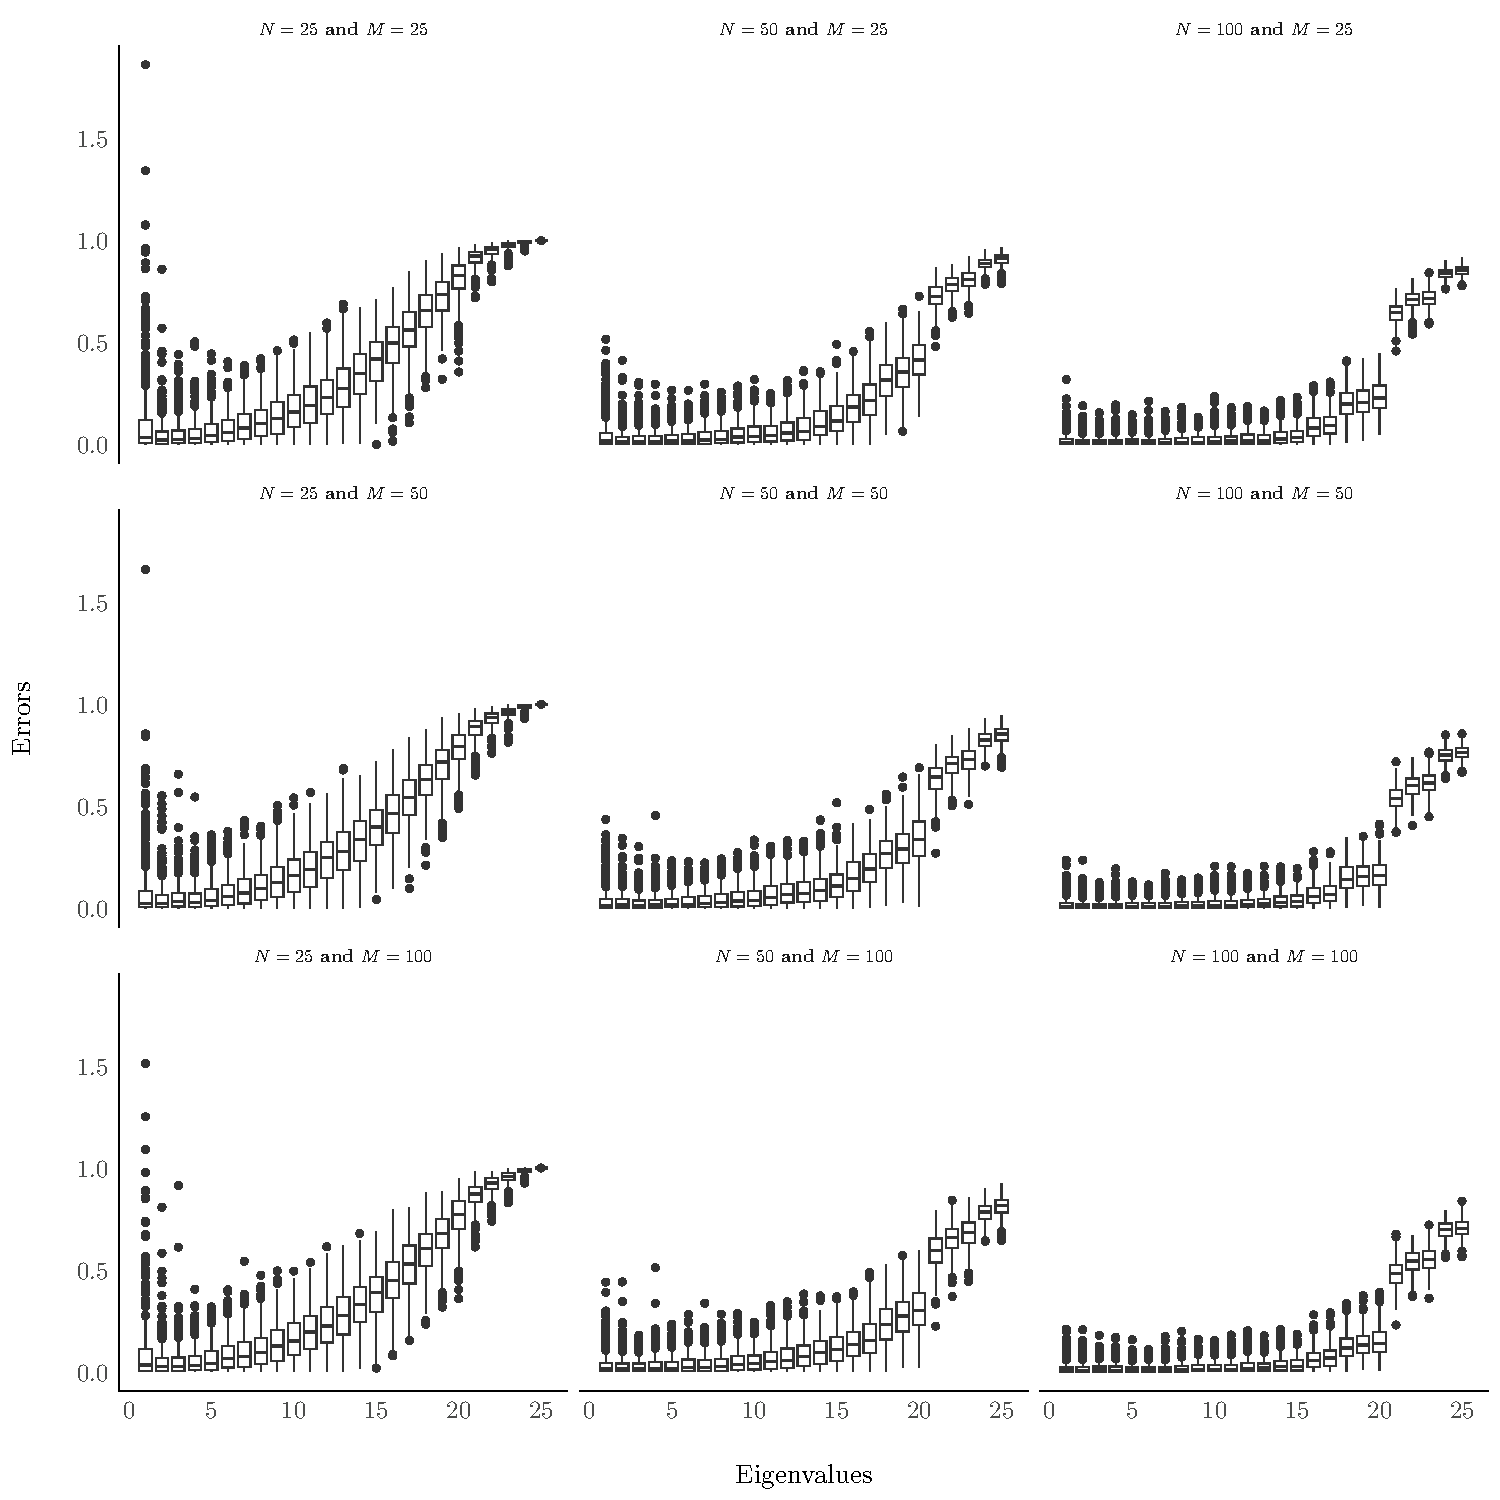
\includegraphics[width=0.95\textwidth]{figures/ncomp.pdf}
    \caption{Boxplots of the estimation errors of the eigenvalues. We estimated $5$ (red boxplots) and $10$ (blue boxplots) components for each of $p = 5$ univariate feature. The number of multivariate eigencomponents that are estimated is $25$. $N$ is the number of observations, $S$ is the number of sampling points per curve. We run $500$ simulations.}
    \label{fig:ncomp}
\end{figure}
Figure \ref{fig:npc_estim} presents the estimation of the number of components retained across $500$ simulation scenarios for a fixed percentage of variance explained. The red dots represent the number of components that should be retained for $\alpha\%$ of variance explained ($50\%, 70\%, 90\%, 95\%$ and $99\%$), considering an exponential decay of the eigenvalues as defined in equation \eqref{eq:npc}. Additionally, the size of the black dots indicates the frequency of selection for each component over the $500$ simulations. For example, for the panel where $N = 25$ and $S = 25$, and for a proportion of variance explained $\alpha = 0.5$, for approximately $200$ simulations over $500$, two multivariate components were required while for around $300$ simulations over $500$ only one multivariate component was required to explain $50\%$ of the variance. Notably, the number of components appears to be consistently underestimated for various combinations of the number of observations $N$, number of sampling points $S$, and desired percentage of variance explained $\alpha\%$. These findings may hold considerable significance for practitioners.
\begin{figure}
     \centering
    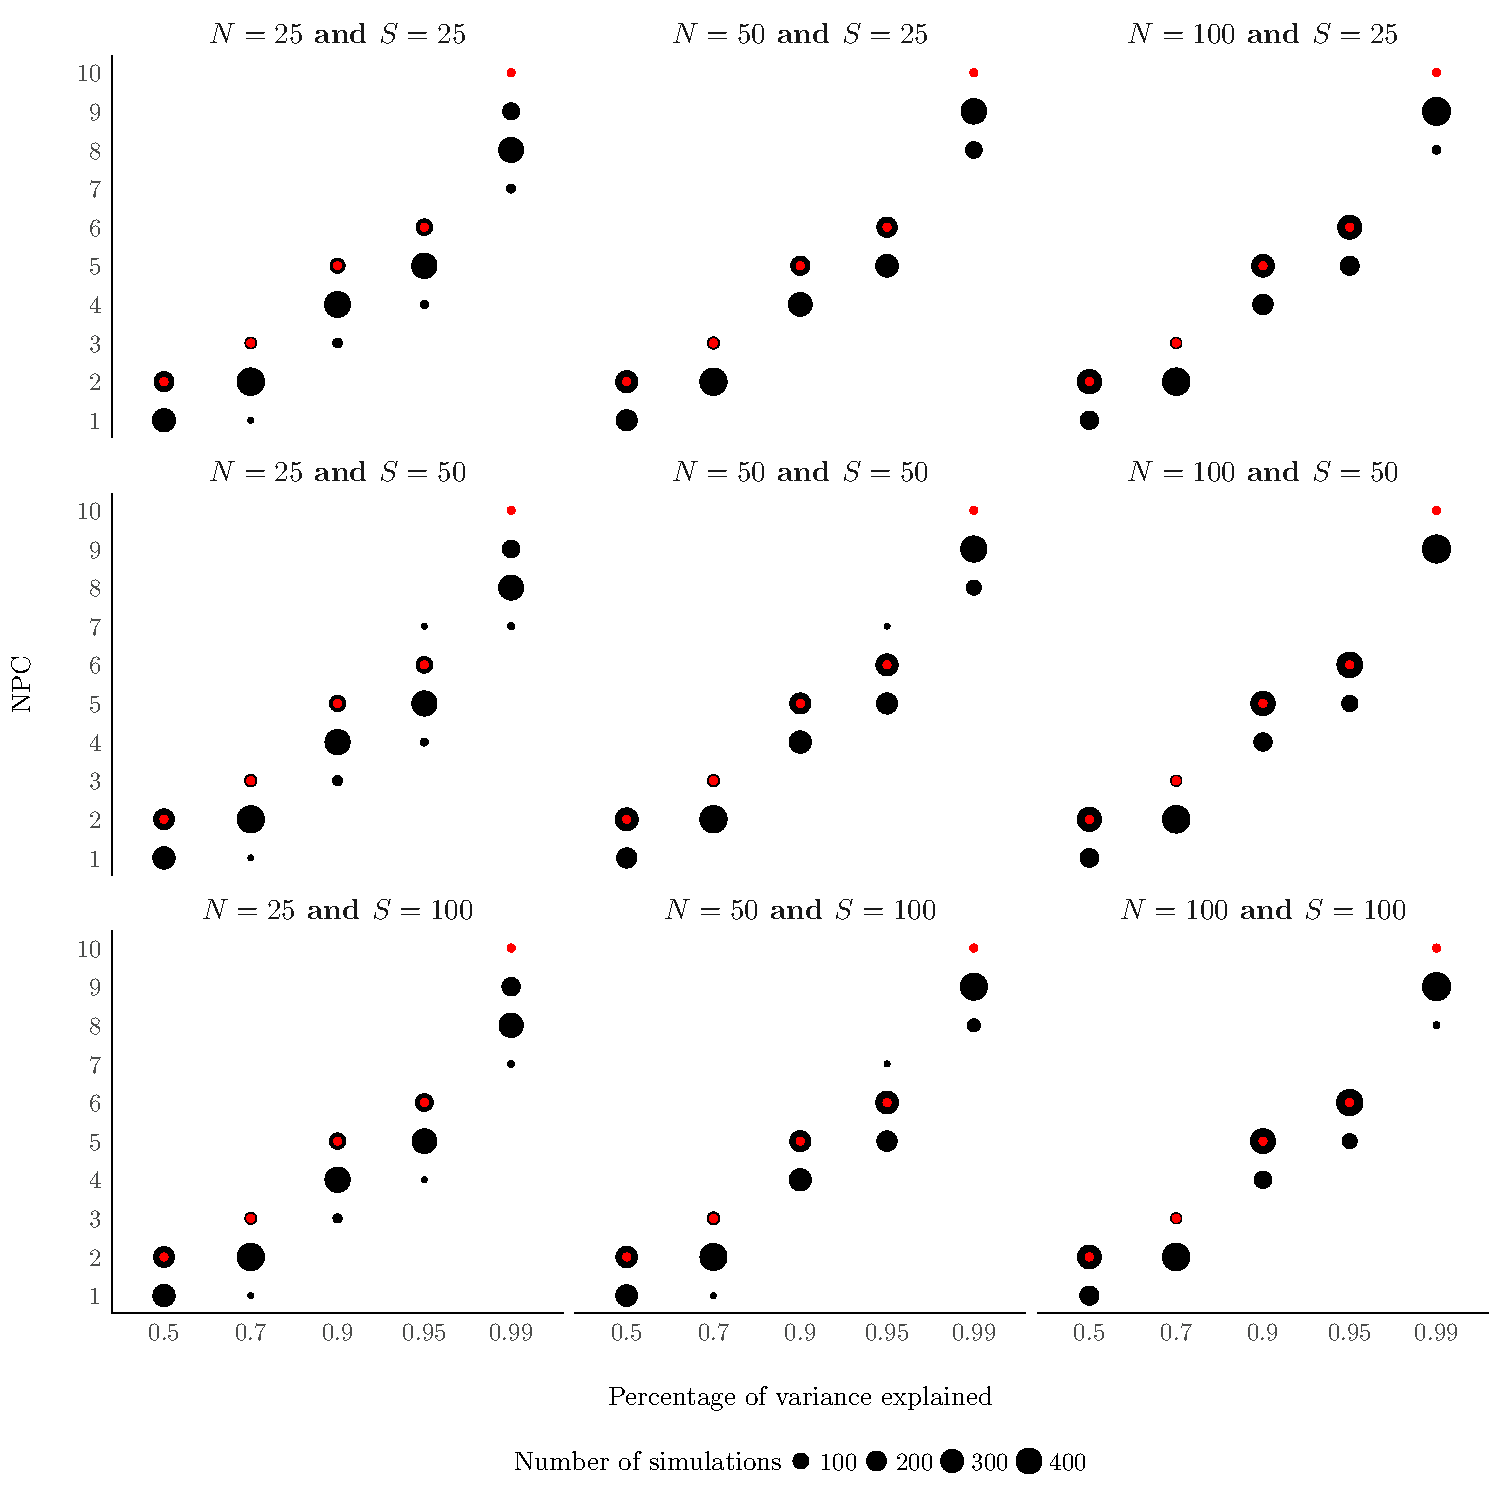
\includegraphics[width=0.95\textwidth]{figures/npc_estim.pdf}
    \caption{The size of the black dots represents the number of times the number of components has been selected over $500$ simulations. The red dots are the true number of components given the percentage of variance explained. $N$ is the number of observations, $S$ is the number of sampling points per curve. The size of the black dots is continuous.}
    \label{fig:npc_estim}
\end{figure}

% section simulation (end)

\section{Conclusion} % (fold)
\label{sec:conclusion}

\cite{happMultivariateFunctionalPrincipal2018} presents a general methodology to estimate principal components for a set of multivariate functional data defined on, possibly, different dimensional domains. Their approach, based on the decomposition of the covariance of each univariate feature, allows easy inference of the components.

We conducted a simulation study, and the obtained results highlight two important findings. Firstly, although utilizing only a few univariate components may yield a substantial number of multivariate components, their accuracy is notably limited. Secondly, relying on the percentage of variance explained as a criterion for selecting the number of components may result in an underestimation of this number. We, therefore, advise practitioners to exercise caution when determining the number of estimated components require in their analysis. It is prudent to refrain from utilizing more than $M_{-}$ estimated multivariate components. Additionally, we strongly recommend conducting simulations that closely resemble the characteristics of the actual data to select the appropriate number of components based on the percentage of variance explained criterion.

% section conclusion (end)





